
\documentclass[a4paper,11pt]{article}
\usepackage[a4paper, margin=8em]{geometry}

% usa i pacchetti per la scrittura in italiano
\usepackage[french,italian]{babel}
\usepackage[T1]{fontenc}
\usepackage[utf8]{inputenc}
\frenchspacing 

% usa i pacchetti per la formattazione matematica
\usepackage{amsmath, amssymb, amsthm, amsfonts}

% usa altri pacchetti
\usepackage{gensymb}
\usepackage{hyperref}
\usepackage{standalone}

% imposta il titolo
\title{Appunti Comunicazioni Numeriche}
\author{Luca Seggiani}
\date{2026}

% imposta lo stile
% usa helvetica
\usepackage[scaled]{helvet}
% usa palatino
\usepackage{palatino}
% usa un font monospazio guardabile
\usepackage{lmodern}

\renewcommand{\rmdefault}{ppl}
\renewcommand{\sfdefault}{phv}
\renewcommand{\ttdefault}{lmtt}

% disponi il titolo
\makeatletter
\renewcommand{\maketitle} {
	\begin{center} 
		\begin{minipage}[t]{.8\textwidth}
			\textsf{\huge\bfseries \@title} 
		\end{minipage}%
		\begin{minipage}[t]{.2\textwidth}
			\raggedleft \vspace{-1.65em}
			\textsf{\small \@author} \vfill
			\textsf{\small \@date}
		\end{minipage}
		\par
	\end{center}

	\thispagestyle{empty}
	\pagestyle{fancy}
}
\makeatother

% disponi teoremi
\usepackage{tcolorbox}
\newtcolorbox[auto counter, number within=section]{theorem}[2][]{%
	colback=blue!10, 
	colframe=blue!40!black, 
	sharp corners=northwest,
	fonttitle=\sffamily\bfseries, 
	title=~\thetcbcounter: #2, 
	#1
}

% disponi definizioni
\newtcolorbox[auto counter, number within=section]{definition}[2][]{%
	colback=red!10,
	colframe=red!40!black,
	sharp corners=northwest,
	fonttitle=\sffamily\bfseries,
	title=~\thetcbcounter: #2,
	#1
}

% U.D.M
\newcommand{\amp}{\ensuremath{\mathrm{A}}}
\newcommand{\volt}{\ensuremath{\mathrm{V}}}
\newcommand{\meter}{\ensuremath{\mathrm{m}}}
\newcommand{\second}{\ensuremath{\mathrm{s}}}
\newcommand{\farad}{\ensuremath{\mathrm{F}}}
\newcommand{\henry}{\ensuremath{\mathrm{H}}}
\newcommand{\siemens}{\ensuremath{\mathrm{S}}}

% circuiti
\usepackage{circuitikz}
\usetikzlibrary{babel}

% disegni
\usepackage{pgfplots}
\pgfplotsset{width=10cm,compat=1.9}

% disponi codice
\usepackage{listings}
\usepackage[table]{xcolor}

\lstdefinestyle{codestyle}{
		backgroundcolor=\color{black!5}, 
		commentstyle=\color{codegreen},
		keywordstyle=\bfseries\color{magenta},
		numberstyle=\sffamily\tiny\color{black!60},
		stringstyle=\color{green!50!black},
		basicstyle=\ttfamily\footnotesize,
		breakatwhitespace=false,         
		breaklines=true,                 
		captionpos=b,                    
		keepspaces=true,                 
		numbers=left,                    
		numbersep=5pt,                  
		showspaces=false,                
		showstringspaces=false,
		showtabs=false,                  
		tabsize=2
}

\lstdefinestyle{shellstyle}{
		backgroundcolor=\color{black!5}, 
		basicstyle=\ttfamily\footnotesize\color{black}, 
		commentstyle=\color{black}, 
		keywordstyle=\color{black},
		numberstyle=\color{black!5},
		stringstyle=\color{black}, 
		showspaces=false,
		showstringspaces=false, 
		showtabs=false, 
		tabsize=2, 
		numbers=none, 
		breaklines=true
}

\lstdefinelanguage{javascript}{
	keywords={typeof, new, true, false, catch, function, return, null, catch, switch, var, if, in, while, do, else, case, break},
	keywordstyle=\color{blue}\bfseries,
	ndkeywords={class, export, boolean, throw, implements, import, this},
	ndkeywordstyle=\color{darkgray}\bfseries,
	identifierstyle=\color{black},
	sensitive=false,
	comment=[l]{//},
	morecomment=[s]{/*}{*/},
	commentstyle=\color{purple}\ttfamily,
	stringstyle=\color{red}\ttfamily,
	morestring=[b]',
	morestring=[b]"
}

% disponi sezioni
\usepackage{titlesec}

\titleformat{\section}
	{\sffamily\Large\bfseries} 
	{\thesection}{1em}{} 
\titleformat{\subsection}
	{\sffamily\large\bfseries}   
	{\thesubsection}{1em}{} 
\titleformat{\subsubsection}
	{\sffamily\normalsize\bfseries} 
	{\thesubsubsection}{1em}{}

% disponi alberi
\usepackage{forest}

\forestset{
	rectstyle/.style={
		for tree={rectangle,draw,font=\large\sffamily}
	},
	roundstyle/.style={
		for tree={circle,draw,font=\large}
	}
}

% disponi algoritmi
\usepackage{algorithm}
\usepackage{algorithmic}
\makeatletter
\renewcommand{\ALG@name}{Algoritmo}
\makeatother

% disponi numeri di pagina
\usepackage{fancyhdr}
\fancyhf{} 
\fancyfoot[L]{\sffamily{\thepage}}

\makeatletter
\fancyhead[L]{\raisebox{1ex}[0pt][0pt]{\sffamily{\@title \ \@date}}} 
\fancyhead[R]{\raisebox{1ex}[0pt][0pt]{\sffamily{\@author}}}
\makeatother

\begin{document}
% sezione (data)
\section{Lezione del 15-05-26}

% stili pagina
\thispagestyle{empty}
\pagestyle{fancy}

% testo
\subsection{Sistemi di comunicazione}
Avevamo introdotto in 1.2 i sistemi di comunicazione formati da:
\begin{itemize}
	\item Una data \textit{sorgente} di segnale;
	\item Un \textit{codificatore di sorgente} che riduce la ridondanza del segnale. Chiameremo il suo segnale in uscita $\{b_n\}$;
	\item Un \textit{codificatore di canale} che introduce ridondanza per preparare il segnale al canale. Chiameremo il suo segnale in uscita $\{d_n\}$;
	\item Un \textit{modulatore}, che si occupa effettivamente di pilotare il canale. Questo era il componente che ci mancava da vedere.
\end{itemize}

A valle del modulatore c'era il mezzo di trasmissione vero e proprio, e quindi il \textit{demodulatore}, il {decodificatore di canale} e il \textit{decodificatore di sorgente} che ricostruivano il segnale originale della sorgente.

Ora, $\{b_n\}$ (monte codificatore di canale) ha rate $R_b$, mentre $\{d_n\}$ (valle codificatore di canale) ha rate $R_d$. Questi rate sono legati dalla solita equazione:
$$
k T_b = n T_d, \quad \frac{T_d}{T_b} = \frac{k}{n} \implies \frac{R_b}{R_d} = \frac{k}{n} = r
$$
Quando si usa una codifica a blocco di rate $r$.

\subsubsection{Struttura del demodulatore}
Veniamo allora alla struttura del componente demodulatore.

\begin{center}
	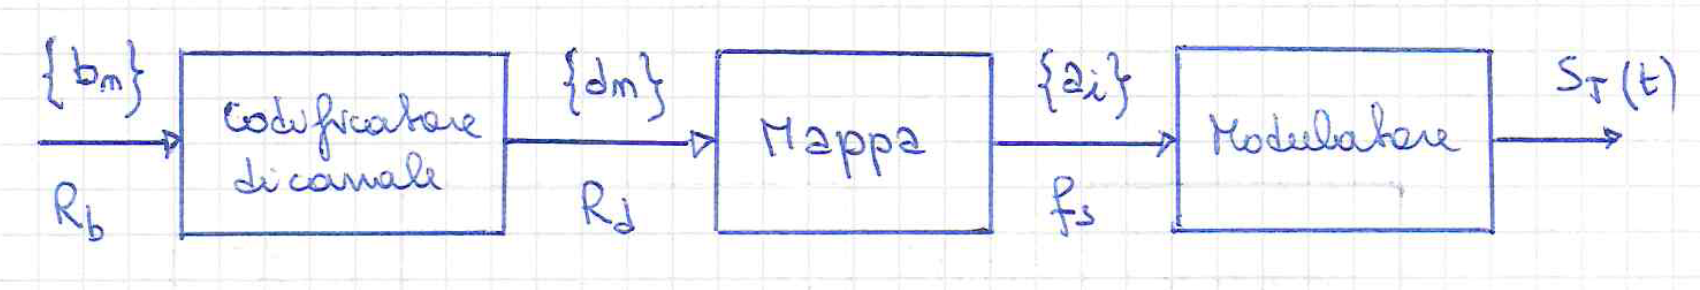
\includegraphics[scale=0.25]{../figures/cod_map_mod.png}
\end{center}

Questo prenderà in ingresso l'uscita del decodificatore di canale $\{d_n\}$, che andrà in ingresso a:
\begin{itemize}
\item Un modulo detto \textbf{mappatore}, la cui uscita chiamiamo $\{a_i\}$. Il mappatore ha il compito di trasformare lo spazio dei simboli $\{d_n\}$ ad un alfabeto $M$ di $2^Q$, dove $Q$ è il numero di bit che compongono il simbolo $d_n$.

Il periodo $T_s$ del segnale in uscita dal mappatore è:
$$
T_s = Q T_d = \log_2 (\# M) T_d, \quad R_s = \frac{1}{T_s} = \frac{R_d}{\log_2(\# M)} = \frac{R_d}{Q}
$$
dove $\# M$ è il numero di simboli dell'alfabeto (equivalentemente $2^Q$). Solitamente la frequenza del numero di simboli in uscita $\{a_i\}$ si misura in \textit{baud}. 

Il vantaggio dato dall'uso di un mappatore è dato dal fatto che si riesce a trasmettere la stessa informazione a frequenza minore, in quanto invece di trasmettere bit a periodo $T_d$, trasmettiamo simboli (dati dall'alfabeto $M$) a periodo $T_s$, e solitamente:
$$
T_s > T_d
$$

\item Un filtro di interpolazione $g_T(t)$, la cui uscita chiamiamo $S_T(t)$. Questa avrà formula data dal filtraggio dei simboli mappati:
$$
S_T(t) = \sum_i a_i g_T (t - i T_s)
$$
Questo riporta il segnale campionato in un segnale a tempo continuo.

L'interpolatore più semplice che possiamo realizzare, abbiamo visto, è quello a mantenimento:
$$
g_T(t) = \mathrm{rect} \left( \frac{t}{T_s} \right) \implies S_T(t) = \sum_i a_i \mathrm{rect} \left( \frac{t - i T_s}{T_s} \right)
$$
In questo caso la densità spettrale di potenza della $S_T(t)$ ha la forma di una $\mathrm{sinc}(f T_S)$, che sappiamo si annulla per la prima volta a $\frac{1}{T_s}$. In confronto, il segnale $\{d_n\}$ campionato a frequenza $R_d$ aveva banda che si annullava per la prima volta a $\frac{1}{T_d}$. Come avevamo detto:
$$
T_s > T_d \implies \frac{1}{T_s} < \frac{1}{T_d}
$$
e quindi la banda in uscita dal mappatore è minore di quella in uscita dal codificatore di canale: abbiamo ridotto l'utilizzo di banda dato dall'introduzione di ridondanza al codificatore di canale.

Il contro di questo approccio è che l'uscita $\{a_i\}$ è più suscettibile al rumore (come vedremo in seguito, la $S_T(t)$ è veramente un processo aleatorio), per cui il sistema di comunicazione è meno robusto. 

\item Un modulatore a radiofrequenza, dalla risposta temporale $\cos(2 \pi f_0 t)$, la cui uscita chiamiamo $S_T^{(RF)}(t)$. Questo avrà il compito d prendere il segnale in banda base, modularlo ad una $f_0$ in spettro di frequenza radio, e quindi inviare il segnale ottenuto all'antenna. L'equazione dell'uscita è:
$$
S_T^{(RF)}(t) = S_T(t) \cos (2 \pi f_0 t)
$$
\end{itemize}

Visto che non conosciamo in anticipo il segnale che vogliamo trasmettere, l'uscita in banda base $S_T(t)$ rappresenta effettivamente un \textit{processo aleatorio}, che vorremo descrivere in termini di media ed autocorrelazione. 

Potremmo considerare il processo come deterministico, e quindi prendere la trasformata:
$$
s_T(t) \rightarrow S_T(f), \quad \text{TCF}
$$
$$
S_T(f) = \sum_i a_i G_T (f) e^{-i 2 \pi f n T_s} = G_T(f) \underbrace{\sum_i a_i e^{- 2 \pi f n T_s}}_\text{TDF}
$$
dove il termine evidenziato è la trasformata discreta della specifica sequenza di $a_i$ (e quindi lo specifico segnale trasmesso), e la $G_T(f)$ è costante. Questa però è una visione solo parziale del sistema: la TDF varia infatti al variare del segnale all'origine, e quindi è meglio trattare il segnale in termini statistici (considerando tutti i possibili segnali trasmessi). 

\subsubsection{Sistemi di comunicazione PAM}
Il tipo di sistema di comunicazione che vedremo sarà quello \textbf{PAM}, da \textit{Pulse Amplitude Modulation}. In breve, questi sistemi sono caratterizzati da impulsi a modulazione di ampiezza, e quindi mappatori a valori discreti (analogici, $\pm k$) e interpolatori a mantenimento.

\subsubsection{Descrizione statistica}
Abbiamo detto che del segnale in uscita dal mappatore $\{a_i\}$ ci interessava la descrizione statistica del primo e del secondo ordine, cioè:
$$
\begin{cases}
	\eta_a = E \{a_i\} \\
	R_a (m) = E \{ a_i a_{i + m} \}
\end{cases}
$$
\begin{itemize}
\item \textbf{\textsf{Valor medio}} \\
Questa è banale se si assume che ogni simbolo è equiprobabile, in quanto:
$$
\eta_a = E \{a_i\} = \sum_{l = 1}^M P_r(a_i = a^{(l)}) a^{(l)} = \frac{1}{M} \sum_{l = 1}^M a^{(l)}
$$
Per questo motivo nella PAM si scelgono costellazioni simmetriche, cioè tali che:
$$
\frac{1}{M} \sum_{l = 1}^M a^{(l)} = 0
$$
\item \textbf{\textsf{Autocorrelazione}} \\
L'autocorrelazione dipende dal valore $m$ fornito:
$$
R_a(m) =
\begin{cases}
	E \{a_i^2\}, \quad m = 0
	E \{a_i a_{i + m}\}, \quad m \neq 0
\end{cases}
$$
Dividiamo oltre. Facendo l'ipotesi di avere un \textit{interleaver} (visto in 23.0.2), possiamo assumere che i simboli $a_i$ siano fra di loro incorrelati, per cui:
\begin{itemize}
	\item 
$
E\{ a_i^2 \} = \sum_{l = 1}^M P_r \left(a_i = a^{(l)}\right) \left(a^{(l)}\right)^2
$
\item
$
E\{ a_i a_{i + m} \} = E\{a_i\}E\{a_{i + m}\} = \eta_a^2
$
\end{itemize}

Riprendendo il fatto che la costellazione è simmetrica, si ottiene:
$$
R_a(m) =
\begin{cases}
	E\{a_i^2\}, \quad m = 0 \\
	0, \quad m \neq 0
\end{cases}
= E \{ a_i^2 \} \delta(m)
$$
cioè si ritorna alla $\delta$.

Notiamo inoltre che, visto che il valor medio è nullo, vale la solita relazione per il valore quadratico medio:
$$
E\{a_i^2\} = \sigma^2_a - \eta_a^2 = \sigma^2_a 
$$
per cui vale anche:
$$
R_a(m) = \sigma^2_a \delta(m)
$$

Notiamo che solitamente $\sigma_a^2$ si definisce come:
$$
\sigma_a^2 = E \{ a_i^2 \} = \frac{(\# M)^2 - 1}{3}
$$

\end{itemize}

\subsubsection{Descrizinoe in spettro}
A questo punto vogliamo calcolare la descrizione in spettro di frequenza, che non ci soddisfaceva in dominio determinstico, in quanto risultava dipendente dai simboli $a_i$. Prendiamo quindi la densità spettrale di potenza del segnale in uscita dall'interpolatore (cioè in banda base) come:
$$
S_S(f) = \frac{1}{T_s} S_a(f) | G_T(f) |^2
$$
Resta da calcolare la $S_a(f)$. Questa si avrà da:
$$
S_a(f) = \sum_m R_a(m) e^{-i 2 \pi m f T_s} = \sigma_a^2
$$
per cui:
$$
S_S(f) = \frac{1}{T_s} S_a(f) | G_T(f) |^2 = \frac{1}{T_s} \sigma_a^2 | G_T(f) |^2
$$

\subsubsection{Considerazioni di potenza}
La potenza $P_S$ del segnale sarà l'integrale della densità di potenza:
$$
P_S = \int_{-\infty}^{\infty} S_S(f) \, df = \frac{\sigma^2}{T_S} \underbrace{\int_{-\infty}^{\infty} | G_T(f) |^2 \, df}_{E_{g_T}} = \frac{\sigma_a^2}{T_s} E_{g_T}
$$
dove la $E_{g_T}$ sarà la potenza del filtro di interpolazione. Nel caso più semplice, dove l'interpolatore è a mantenimento, questa vale $T_s$, per cui la potenza risulta $\sigma_a^2$.

\subsubsection{Considerazioni energetiche}
Data una definizione della potenza del segnale, possiamo dare un indicazione dell'energia usata per simbolo: 
$$
E_s = P_s T_s = \sigma_a^2 E_{g_T} = \frac{(\# M)^2 - 1}{3} E_{g_T}
$$

Questo discorso può essere ripetuto all'indietro, permettendoci di trovare l'energia usata per bit dal codificatore di canale:
$$
E_d = \frac{E_s}{Q} = \frac{\sigma_a^2}{\log_2 (\# M)} E_{g_T}
$$
e l'energia usata per bit dal codificatore di sorgente:
$$
E_b = \frac{1}{r} E_d = \frac{\sigma_a^2}{r \log_2(\# M)} E_{g_T}
$$

\subsubsection{Considerazioni finali sulla banda}
Avevamo detto che per la banda al trasmettitore potevamo dire:
$$
B_s = \frac{1}{T_s} = \frac{1}{\log(\# M) T_d} = \frac{R_d}{\log_2 (\# M)} = \frac{R_d}{Q}
$$
Interroghiamoci adesso sulla dipendeza dal periodo al codificatore di sorgente. Avremo che:
$$
R_d = \frac{R_b}{r} \implies B_s = \frac{R_b}{r \log_2(\# M)}
$$

Questa equazione ci è utile in quanto enuncia esattamente la dipendenza dell abanda dai parametri di codifica:
\begin{itemize}
	\item $R_b$ è la frequenza di bit in uscita dal codificatore si sorgente, che prendiamo per fissa; 
	\item $r$ è il rate del codice: diminuendolo (e quindi portando meno bit dati per bit totali) si aumenta la banda usata;
	\item $\log_2(\# M)$ indica la dimensione dell'alfabeto: aumentandola, la si diminuisce la banda usata.
\end{itemize}

Se il segnale sorgente è campionato a frequenza $2B$ (da Nyquist), il risultato è che la banda di tramissione è:
$$
B_s = \frac{\log_2 (l)}{r \log_2 (\#M)} (2B)
$$
dove la $l$ è la lunghezza della parola di codifica di un singolo campione.

\end{document}
